\section*{Topologische Überlegungen}\addcontentsline{toc}{section}{Topologische Überlegungen}\label{sec:topologie}
\fancyhead[RO]{Topologische Überlegungen}
% \fancyhead[LO]{}

Die aktuelle Form ist durch den Absturz der Raumstation mitverursacht, und vermutlich ist die gewissermaßen "`flache"' Struktur, die wir bei den bisherigen Rekunstruktionsphasen ausgemacht haben, eine zweidimensionale Projektion der eigentlich mehrdimensionalen Raumstation. Darauf gehen wir hier etwas genauer ein.

Wir haben gesehen, dass sich \ceva{clamp} und \ceva{core} berühren bzw. über eine Einstein-Rosen-Brücke verbunden sind. Daraus folgern wir eine (ursprünglich, zukünftig) ringförmige Anordnung der Ringe; vgl  \cref{fig:ringring}.

\begin{figure}[ht!]
    \centering
    \documentclass{standalone}
\usepackage{tikz}
\usetikzlibrary{decorations, decorations.text}
\usepackage{calc}
\usepackage{xcolor}
\usepackage{fontspec}
\newcommand{\ceva}[1]{~{\fontspec{[ceva-c2.ttf]}#1}}
\definecolor{eins}{HTML}{e7e7e8}   %% Ring 1 "core"     - weiß - Mittelpunkt, Ring um Mittelpunkt
\definecolor{zwei}{HTML}{ed1c24}   %% Ring 2 "com"      - rot -  "Fenster" innen
\definecolor{drei}{HTML}{fbad18}   %% Ring 3  "culture" - orange - fünf Module, quasi invertiert
\definecolor{vier}{HTML}{74c043}   %% Ring 4  "creactiv" - grün -  vier Module
\definecolor{fuenf}{HTML}{0089d0}  %% Ring 5 "cience"  - cyan (blau) - drei Module mit "Strich"
\definecolor{sechs}{HTML}{11357e}  %% Ring 6 "carbon" -  indigo - viele "Fenster" außen
\definecolor{sieben}{HTML}{000000} %% Ring 7 "clamp" -  schwarz, c-förmig
\definecolor{cbase}{HTML}{222222}  %% Körper der Raumstation    
\begin{document}
%% c-base logo nachgebaut von penta.
%% alles nur geschätze Winkel und Abstände :/
%% um den code zu verstehen, einfach mal einzelne Teile auskommentieren und wieder einkommentieren (ctrl-#) und dann mal \draw[white] durch \draw[red] ersetzen, dann sieht man, was was ist.
%% viel Spaß damit.
\tikzset{
  pics/carc/.style args={#1:#2:#3:#4}{
    code={
      \draw[postaction={decorate, decoration={text along path, raise=-2pt, text align={align=center}, text={\ceva{#4}}, reverse path}}] (#1:#3) arc(#1:#2:#3);
    }
  }
}%
    \begin{tikzpicture}
        \draw[gray, line width=50pt] (0:0) circle (3);
        \foreach [count=\i] \ring/\color in
            {core/eins,com/zwei,culture/drei,creactiv/vier,cience/fuenf,carbon/sechs,clamp/sieben}
            {%
                \draw[color=\color!50,line width=45pt] (0:0) pic{carc=\i*51.418-25:\i*51.418+25:3:\ring};
            }%
    \end{tikzpicture}
\end{document}

    \caption{Ringförmige Anordnung der \ring{Ringe}}
    \label{fig:ringring}
\end{figure}

Eine \emph{ringförmige Anordnung von Ringen }ist geometrisch darstellbar auf einer Oberfläche, die entsteht, wenn ein Kreis um einen Kreis (also quasi ein \ring{Ring} um einen \ring{Ring}) rotiert. Diese Figur ist der Rotationstorus. \cref{fig:torusweiss}  zeigt zur Veranschaulichung ein toroidales Polyeder mit $14\times 14$ Flächen.  

\begin{figure}[ht!]
    \centering
    \documentclass{standalone}
\usepackage{xcolor}
\usepackage[svgnames]{pstricks}
\usepackage{pst-solides3d}
\definecolor{eins}{HTML}{e7e7e8}   %% Ring 1 "core"     - weiß - Mittelpunkt, Ring um Mittelpunkt
\definecolor{zwei}{HTML}{ed1c24}   %% Ring 2 "com"      - rot -  "Fenster" innen
\definecolor{drei}{HTML}{fbad18}   %% Ring 3  "culture" - orange - fünf Module, quasi invertiert
\definecolor{vier}{HTML}{74c043}   %% Ring 4  "creactiv" - grün -  vier Module
\definecolor{fuenf}{HTML}{0089d0}  %% Ring 5 "cience"  - cyan (blau) - drei Module mit "Strich"
\definecolor{sechs}{HTML}{11357e}  %% Ring 6 "carbon" -  indigo - viele "Fenster" außen
\definecolor{sieben}{HTML}{000000} %% Ring 7 "clamp" -  schwarz, c-förmig
\definecolor{cbase}{HTML}{222222}  %% Körper der Raumstation    
\begin{document}

%% https://ftp.tu-chemnitz.de/pub/tex/graphics/pstricks/contrib/pst-solides3d/doc/pst-solides3d-doc.pdf

\begin{pspicture}(-4,-4)(4,4)
    \psset{Decran=20,viewpoint=5 11 25}
    \pstVerb{/iface 0 store}%
    \psSolid[
        r1=3,r0=2,
        object=tore,
        ngrid=14 14,
        RotY=30]
\end{pspicture}


\end{document}
    \caption{Ein Toroidales Polyeder imt $14\times 14$T Flächen} Es hat 14  Meridiane und 14 Parallelkreise (angenähert)
    \label{fig:torusweiss}
\end{figure}

Nun stellt sich die Frage, wie die \ring{Ringe} auf so einem Torus angeordnet waren bzw. sein werden bzw. sollen. 

Grundsätzlich sind die \ring{Ringe} Kreisscharen. Es gibt drei verschiedene Gruppen von Kreisscharen auf einem Torus: Parallelkreise, Merididiane und Villarceau-Kreise. 

Parallelkreise würden etwa entstehen durch Schnitte eines gefärbten Torus wie z.B. in \cref{fig:torus-parallele} abgebildet. 

\begin{figure}[ht!]
    \centering
    \documentclass{standalone}
\usepackage{xcolor}
\usepackage[svgnames]{pstricks}
\usepackage{pst-solides3d}
\definecolor{eins}{HTML}{e7e7e8}   %% Ring 1 "core"     - weiß - Mittelpunkt, Ring um Mittelpunkt
\definecolor{zwei}{HTML}{ed1c24}   %% Ring 2 "com"      - rot -  "Fenster" innen
\definecolor{drei}{HTML}{fbad18}   %% Ring 3  "culture" - orange - fünf Module, quasi invertiert
\definecolor{vier}{HTML}{74c043}   %% Ring 4  "creactiv" - grün -  vier Module
\definecolor{fuenf}{HTML}{0089d0}  %% Ring 5 "cience"  - cyan (blau) - drei Module mit "Strich"
\definecolor{sechs}{HTML}{11357e}  %% Ring 6 "carbon" -  indigo - viele "Fenster" außen
\definecolor{sieben}{HTML}{000000} %% Ring 7 "clamp" -  schwarz, c-förmig
\definecolor{cbase}{HTML}{222222}  %% Körper der Raumstation    
\begin{document}

%% https://ftp.tu-chemnitz.de/pub/tex/graphics/pstricks/contrib/pst-solides3d/doc/pst-solides3d-doc.pdf

\begin{pspicture}(-4,-4)(4,4)
    \psset{Decran=20,viewpoint=5 11 25}
    \pstVerb{/iface 0 store}%
    \psSolid[
        hue = 0 1,
        % fcol=48 {iface (green)
        % iface 1 add (orange)
        % iface 2 add (orange)
        % iface 3 add (red) 
        % iface 4 add (red) 
        % iface 5 add (white) 
        % iface 6 add (white) 
        % iface 7 add (black) 
        % iface 8 add (black) 
        % iface 9 add (blue) 
        % iface 10 add (blue) 
        % iface 11 add (blue) 
        % iface 12 add (blue) 
        % iface 13 add (blue) /iface
        % iface 14 add store} repeat,
        r1=3,r0=2,
        object=tore,
        ngrid=14 14,
        RotY=30]
\end{pspicture}


\end{document}
    \caption{Parallelkreise}
    \label{fig:torus-parallele}
\end{figure}

Eine solche Anordnung ist zwar möglich, aber wenig plausibel, da die einzelnen Ringe in diesem Fall eher als Schreiben abgebildet werden würden. Auch ist nicht zu erkennen, wie es beim Absturz der Station dann zu einer konzentrischen Anordnung gekommen sein sollte. 

Eine Anodrnung der \ring{Ringe} als Meridiankreise  zeigt \cref{fig:torus-meridiane}.  
Dabei berühren sich hier im Inneren eben \ceva{core} und \ceva{clamp}; das passt zu unserer Interpretation des Kanons von der Topologie der Station als Torus mit einem innenliegenden Wurmloch. In diesem berühren sich innen \ceva{core} und \ceva{clamp}; außen liegt \ceva{creactiv}. 

\begin{figure}[ht!]
    \centering
        \documentclass{standalone}
\usepackage{xcolor}
\usepackage[svgnames]{pstricks}
\usepackage{pst-solides3d}
\definecolor{eins}{HTML}{e7e7e8}   %% Ring 1 "core"     - weiß - Mittelpunkt, Ring um Mittelpunkt
\definecolor{zwei}{HTML}{ed1c24}   %% Ring 2 "com"      - rot -  "Fenster" innen
\definecolor{drei}{HTML}{fbad18}   %% Ring 3  "culture" - orange - fünf Module, quasi invertiert
\definecolor{vier}{HTML}{74c043}   %% Ring 4  "creactiv" - grün -  vier Module
\definecolor{fuenf}{HTML}{0089d0}  %% Ring 5 "cience"  - cyan (blau) - drei Module mit "Strich"
\definecolor{sechs}{HTML}{11357e}  %% Ring 6 "carbon" -  indigo - viele "Fenster" außen
\definecolor{sieben}{HTML}{000000} %% Ring 7 "clamp" -  schwarz, c-förmig
\definecolor{cbase}{HTML}{222222}  %% Körper der Raumstation    
\begin{document}

%% https://ftp.tu-chemnitz.de/pub/tex/graphics/pstricks/contrib/pst-solides3d/doc/pst-solides3d-doc.pdf

\begin{pspicture}(-4,-4)(4,4)
    \psset{Decran=20,viewpoint=5 11 25}
    \pstVerb{/iface 0 store}%
    \psSolid[
        fcol=48 {iface (green)
        iface 1 add (orange)
        iface 2 add (orange)
        iface 3 add (red) 
        iface 4 add (red) 
        iface 5 add (white) 
        iface 6 add (white) 
        iface 7 add (black) 
        iface 8 add (black) 
        iface 9 add (blue) 
        iface 10 add (blue) 
        iface 11 add (blue) 
        iface 12 add (blue) 
        iface 13 add (blue) /iface
        iface 14 add store} repeat,
        r1=3,r0=2,
        object=tore,
        ngrid=14 14,
        RotY=30]
\end{pspicture}


\end{document}
    \caption{Die \ring{Ringe} als Meridiankreise auf dem Torus}
    \label{fig:torus-meridiane}
\end{figure}


Da der äußerere Äquator (Meridian) \ceva{creactive} enspricht, bedeutet eine Ausweitung der \ceva{creactivität} ein Anschwellen dieses Torus und somit Wachstum der Station; bildlich entspräche das in etwa der Inflation eines Rettungsrings. Dabei ist zu beachten, dass eine Vergrößerung des rotierenden Kreises ohne gleichzeitige Ausweitung des Rototaionsradius im Torus zu einem Verschwinden des innenliegenden Loches führen könnte. Dann wäre die Station gewissermaßen an ihrer eigenen \ceva{creactivität} erstickt.

Unsere Darstellung in \cref{fig:torus-meridiane} zeigt die \ring{Ringe} als Flächen. Tatsächlich sind sie natürlich selbst von höherer Diemension, also ihrerseits Tori. Es sollte sich wirklich um eine Schar von Tori, gewissermaßen um ein Bündel von Ringen, handeln.

Betrachten wir nun die vielleicht interessanteste mögliche Anordnung von Kreisscharen auf einem Torso, nämlich die so genannten Villarceau-Kreise. Sie entstehen geometrisch (paarweise) durch den Schnitt einer deoppelberührenden Ebene mit dem Torso (\cref{fig:villarceaukreise}).

\begin{figure}[ht!]
    \centering
    \includesvg{Torus-vill-point.svg}
    \caption{Villarceau-Kreise \cite{villarceauag2gaeh}}
    \label{fig:villarceaukreise}
\end{figure}

Es lässt sich also eine Schar von Kreisen auf einem Torus finden, die sich nicht schneiden, die perfekt kreisförmig und die untereinander kongruent sind. \cref{fig:villarceautorous} zeigt eine Annäherung, indem hier ein Torus mit $21\times 21$ Flächen belegt wurde.

\begin{figure}[ht!] 
    \centering
            \documentclass{standalone}
\usepackage{xcolor}
\usepackage[svgnames]{pstricks}
\usepackage{pst-solides3d}
\definecolor{eins}{HTML}{e7e7e8}   %% Ring 1 "core"     - weiß - Mittelpunkt, Ring um Mittelpunkt
\definecolor{zwei}{HTML}{ed1c24}   %% Ring 2 "com"      - rot -  "Fenster" innen
\definecolor{drei}{HTML}{fbad18}   %% Ring 3  "culture" - orange - fünf Module, quasi invertiert
\definecolor{vier}{HTML}{74c043}   %% Ring 4  "creactiv" - grün -  vier Module
\definecolor{fuenf}{HTML}{0089d0}  %% Ring 5 "cience"  - cyan (blau) - drei Module mit "Strich"
\definecolor{sechs}{HTML}{11357e}  %% Ring 6 "carbon" -  indigo - viele "Fenster" außen
\definecolor{sieben}{HTML}{000000} %% Ring 7 "clamp" -  schwarz, c-förmig
\definecolor{cbase}{HTML}{222222}  %% Körper der Raumstation    
\begin{document}

%% https://ftp.tu-chemnitz.de/pub/tex/graphics/pstricks/contrib/pst-solides3d/doc/pst-solides3d-doc.pdf

\begin{pspicture}(-4,-4)(4,4)
    \psset{Decran=20,viewpoint=5 11 25}
    \pstVerb{/iface 0 store}%
    \psSolid[
        fcol=48 {iface (green)
        iface 1 add (orange)
        iface 2 add (orange)
        iface 3 add (red) 
        iface 4 add (red) 
        iface 5 add (white) 
        iface 6 add (white) 
        iface 7 add (black) 
        iface 8 add (black) 
        iface 9 add (blue) 
        iface 10 add (blue) 
        iface 11 add (SkyBlue) 
        iface 12 add (SkyBlue) 
        iface 13 add (green) /iface
        iface 14 add store} repeat,
        r1=3,r0=2,
        object=tore,
        ngrid=27 14,
        RotY=30]
\end{pspicture}

\end{document}            
    \caption{Die \ceva{Ringe} als Villarceau-Kreise} Approximation auf einem toroidalen Polyeder mit $21\times21$ Flächen
    \label{fig:villarceautorous}
\end{figure}


Nach \cref{fig:villarceautorous} wären die \ring{Ringe} auf einem Torus in Form verschlungener Bänder angeordnet. Sie winden sich um das Zentrum des Torus und zugleich um den Körper des Torus selbst. 
Es gibt keinen \ring{Ring}, der einen bevorzugten Ort einnimmt. Da sie kongruent sind, sind sie flächen- und längengleich.


Wie bereits oben müssen wir uns die Ringe nicht wie abgebildet vorstellen, sondern ihrerseits eher als eigenständige Tori oder Toroide. Ähnlich wie ein Torus (2D, eine Fläche) aus Villacreau-Kreisen "`zusammengesetzt"' vorgestellt werden kann, kann ein Toroid (3D, ein Körper, gewissermaßen ein "`ausgefüllter"' Torus) aus Scharen von Tori "`zusammengesetzt"' bzw. approximiert werden. Wir müssen uns also wieder die \ring{Ringe} in \cref{fig:villarceautorous} als eigene Tori vorstellen.

Das setzt allerdings voraus, dass die \ring{Ringe} eindeutig abgegrenzt sind gegeneinander: jeder \ring{Ring} schließt sich nach einer vollen Umdrehung um die Mittelachse des Torus. Lässt man diese Bedingung fallen, so kann man sich auch einen Torus vorstellen, bei dem jeder Kreis nach $306^o$ an den jeweils nächsten "`anschließt"', also einen "`verknoteten Torus"' bzw. \cevain{cnoten}, wie gezeigt in \cref{fig:knottedtorus}.

\begin{figure}
    \centering
    \resizebox{0.5\textwidth}{!}{
        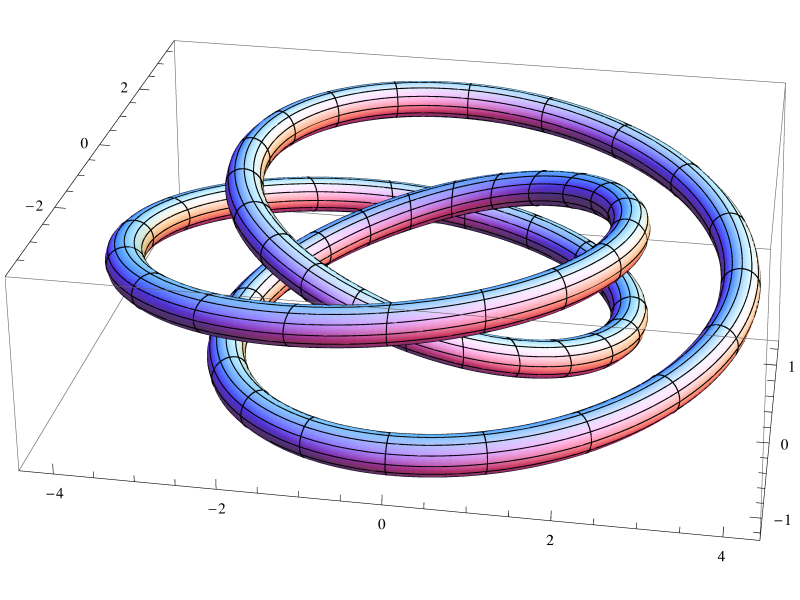
\includegraphics{KnottedTorus.png}
    }
    \caption{Verknoteter Torus \cite{knottedtorus}}
    \label{fig:knottedtorus}
\end{figure}

Dann gäbe es genau einen parallelen Schnitt durch den \cevain{cnoten}, der ein Bild wie \cref{fig:ringring} abgibt, obwohl alle \ring{Ringe} und damit die Station als Ganzes ein einzelner, gewissermaßen siebenfach "`gewickelter"' Torus wäre, nämlich ein Torusknoten.
% Von diesen gibt es widerum verschiedene Formen, 

Angesichts der Bedeutung toroidaler Topologie für Fusionsreaktoren vermuten wir, dass wir hier der Topologie des \ceva{Möbius-band-accelerators} bzw. \ceva{Mino-reactors} bzw. \ceva{Cybernetischen Quecksilber-Reaktors}  auf der Spur sind (vgl.~\cref{sec:core}). 

Die weitere Erforschung dieser Topologie und die möglichen Bedeutungen für die energetische Ausbeute des verschlungenen Miteinanders der sich ergänzenden \ring{Ringe} ist eine Aufgabe ohne Endpunkt.


% Und das ist ein Bild schön genug, dieses Papier zu beschließen.

% \begin{center}
%     \ceva{-- be future compatible --}    
    
%     -- be future compatible --
% \end{center}